\documentclass[10pt,pdf,hyperref={unicode}, dvipsnames]{beamer}
\usepackage[english,russian]{babel}
% \usepackage[T2A,T1]{fontenc}
\usepackage[utf8]{inputenc}
\usepackage{tikz}
\usepackage[unicode]{hyperref}
\usepackage{pgfplots,standalone}
% \usepackage{lmodern}
\pgfplotsset{compat=newest} 
\usetikzlibrary{%
    decorations.pathreplacing,%
    decorations.pathmorphing,%
    patterns,%
    angles,%
    quotes,%
    calc, %
    3d, %
    backgrounds, %
    positioning%
}

% Стиль презентации
\usetheme{Warsaw}

% \setbeamercolor{frametitle right}{fg=white,bg=Brown!85}
% \setbeamercolor{frametitle}{fg=white,bg=Brown!85}
\setbeamercolor{frametitle right}{fg=white,bg=black!85}
\setbeamercolor{frametitle}{fg=white,bg=black!85}

\setbeamertemplate{headline}{}
\setbeamertemplate{footline}{}
\let\Tiny=\tiny % решает проблему со шрифтами в TexLive
\setbeamertemplate
	{footline}{
		\color{black!40!white}
		\quad\hfill
		\insertframenumber/\inserttotalframenumber
		\hfill\vspace{1em}\quad
	} 

\setbeamertemplate{navigation symbols}{}

\beamersetrightmargin{0.5cm} 
\beamersetleftmargin{0.5cm}

\setbeamertemplate{enumerate item}{
	\usebeamercolor[bg]{item projected}
	\raisebox{1pt}{\colorbox{bg}{\color{fg}\footnotesize\bf\insertenumlabel}}%
}
\setbeamercolor{item projected}{bg=black,fg=white}

\setbeamertemplate{itemize item}{%
	\usebeamercolor[bg]{item projected}%
	\raisebox{1pt}{{\color{bg}\footnotesize$\bf\square$}}%
}
\setbeamercolor{item projected}{bg=black,fg=white}
\setbeamercolor{title}{bg=black,fg=white}

\title[Магнитооптическая активность теллуритных стёкол]{Исследование магнитооптических свойств высокочистых теллуритных стёкол}

\author{%
	Геликонова В.Г., %
	Платонова М.В., %
	Сарафанов Ф.Г. %
}

\institute{Радиофизический факультет ННГУ, 420 группа}

\date{Нижний Новгород, 2017}

\begin{document}  

%%%%%%%%%%%%%%%%%%%%%%%%%%%%%%%%%%%%%%%%%%%%%%%%%%%%%%%%%%%%%
\begin{frame}[plain]
	\centering
	\vspace{2cm}
	\begin{beamercolorbox}[sep=8pt,center]{title}
		\bf\usebeamerfont{title}\inserttitle
	\end{beamercolorbox}
	\vspace{0.5cm}
	\normalsize \textbf{Работу выполнили:}\\
	\large\insertauthor\\ 
	\vspace{0.5cm}
	\normalsize{\textbf{Научный руководитель:}\\}
	\large{Яковлев А.И.}
	\vfill
	\small{Нижний Новгород -- 2017}
\end{frame}
%%%%%%%%%%%%%%%%%%%%%%%%%%%%%%%%%%%%%%%%%%%%%%%%%%%%%%%%%%%%%
% \begin{frame}[t]
%   \frametitle{Содержание}
%   \tableofcontents
% \end{frame}
%%%%%%%%%%%%%%%%%%%%%%%%%%%%%%%%%%%%%%%%%%%%%%%%%%%%%%%%%%%%%
\section{Цели и актуальность}
\begin{frame}[t]
	\frametitle{Цели и актуальность}
	\textbf{Цели}\\
	\begin{enumerate}
		\item Ознакомиться с некоторыми понятиями физической оптики
		\item Исследовать магнитооптические свойства теллуритных стёкол (Определить постоянную Верде)
		\item Обработать экспериментальные  результаты и сделать оценку длины образца, пригодного для использования в изоляторах Фарадея 
		при характерных длине волны и напряженности магнитного поля
		% для поля $B=3.5$ Тл и длины волны $\lambda=$1.8 мкм
	\end{enumerate}
	\textbf{Актуальность}\\
	\begin{enumerate}
		\item Теллуритные стекла обладают магниоптической активностью и могут быть использованы в изоляторах и вращателях Фарадея
		\item Теллуритные стекла обладают широким спектром пропускания (0.4--5.5  мкм) %(спектр)
		\item Возможно изготовление образцов с большой апертурой (до 10 см)
		% \item Из теллуритных стекол возможно изготовление волокон
		\item Вариация состава теллуритного стекла позволяет изменять постоянную Верде
	\end{enumerate}
\end{frame}
%%%%%%%%%%%%%%%%%%%%%%%%%%%%%%%%%%%%%%%%%%%%%%%%%%%%%%%%%%%%%
\section{Теоретическая часть}
\begin{frame}[t]
	\subsection{Понятие поляризации}
	\frametitle{Понятие поляризации}
	\begin{enumerate}
		\item \textbf{Поляризация света} -- свойство световой волны, заключающееся в  ориентации векторов напряженности электрического и магнитного полей в плоскости, перпендикулярной волновому вектору $\vec{k}$
		\item Плоскость, образованную векторами $\vec{E}$ и $\vec{k}$ ,называют \textbf{плоскостью поляризации}
	\end{enumerate}
	\begin{gather*}
		\begin{cases} 
			E_x = E_1\cos\left(-kz+\omega t+ \varphi_1\right) \\
			E_y = E_2\cos\left(-kz+\omega t+ \varphi_2\right) \\
			E_z = 0
		\end{cases}
		\quad\Rightarrow\quad
		\frac{E_x^2}{E_1^2}-\frac{2E_xE_y}{E_1E_2}\cos\delta+\frac{E_y^2}{E_2^2}=\sin^2\delta
	\end{gather*}
	\begin{center}
		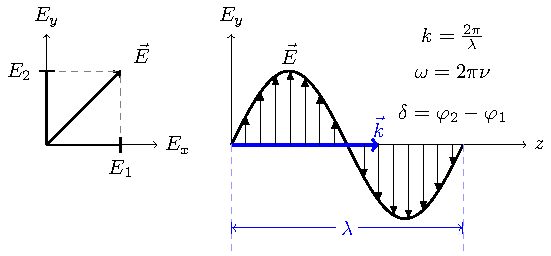
\includegraphics[width=0.7\textwidth]{images/polarisation}
	\end{center}
\end{frame}

%%%%%%%%%%%%%%%%%%%%%%%%%%%%%%%%%%%%%%%%%%%%%%%%%%%%%%%%%%%%%

\begin{frame}
	\begin{columns}
		\begin{column}{0.7\textwidth}
			\begin{enumerate}
				\item Если $\delta=0, \pi$, то
				      \begin{equation*}				
					      \frac{E_x}{E_1}\pm\frac{E_y}{E_2}=0
				      \end{equation*}
				      -- \textbf{линейная} поляризация.
				      \vspace{1em}
				\item Если $\delta=\frac{\pi}{2}$, то\\
				      \begin{equation*}				
					      \frac{E_x^2}{E_1^2}+\frac{E_y^2}{E_2^2}=1				
				      \end{equation*}
				      -- \textbf{эллиптическая} поляризация, которая при $E_1=E_2 \equiv E'$ переходит в \textbf{круговую}:
				      \begin{equation*}				
					      E_x^2+E_y^2=E'^2
				      \end{equation*}
			\end{enumerate}
			C понятием поляризации тесно связано явление \textbf{двойного лучепреломления}.
		\end{column}
		\begin{column}{0.3\textwidth}
			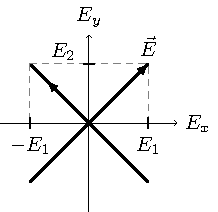
\includegraphics[width=\textwidth]{images/linear_polarisation}\\
			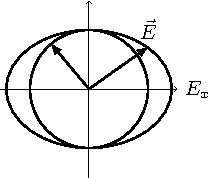
\includegraphics[width=\textwidth]{images/elleptical_polarisation}
		\end{column}
	\end{columns}
\end{frame}

%%%%%%%%%%%%%%%%%%%%%%%%%%%%%%%%%%%%%%%%%%%%%%%%%%%%%%%%%%%%%

\begin{frame}[t]
	\subsection{Понятие двулучепреломления}
	\frametitle{Понятие двулучепреломления}
	\begin{enumerate}
		\item \textbf{Двойное лучепреломление} — раздвоение светового луча при прохождении через анизотропную среду, обусловленное зависимостью показателя преломления от поляризации волны и ориентации волнового вектора.\vspace{-1em}
		      \begin{figure}[tb]
			      \centering
			      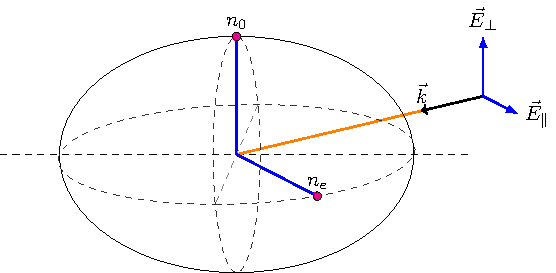
\includegraphics[width=0.8\textwidth]{images/double}
		      \end{figure}
		\item Вращение плоскости поляризации есть проявление \textbf{кругового двулучепреломления }. В этом случае обыкновенная и необыкновенная волны будут поляризованы циркулярно.
	\end{enumerate}
	
	
\end{frame}

%%%%%%%%%%%%%%%%%%%%%%%%%%%%%%%%%%%%%%%%%%%%%%%%%%%%%%%%%%%%%

\begin{frame}[t]
	\begin{enumerate}
		\item \textbf{Круговое двулучепреломление}. Предположим, что угол поворота поляризации зависит от $z$ как
		      $\Theta=-\alpha z$. Тогда можно показать, что волну с повернувшейся поляризацией можно представить как суперпозицию поляризованных по левому ($L$) и правому ($R$) кругу волн, и для них
		      \begin{gather*}
			      v_L=\frac{\omega}{k-\alpha},
			      \quad
			      v_R=\frac{\omega}{k+\alpha},
			      \quad
			      n_L=\frac{c}{v_L},
			      \quad
			      n_R=\frac{c}{v_L}
		      \end{gather*}
		      откуда выражается
		      \begin{equation*}
			      \alpha=\frac{\omega}{2c}(n_L-n_R)
		      \end{equation*}
		\item В магнитном поле у вещества существуют \textbf{собственные частоты} ($\omega_0\pm\Omega$),
		      и по Френелю это и есть причина поворота поляризации: сложение двух таких циркулярно поляризованных волн даст волну с повернутой линейной поляризацией
		      \begin{equation*}
			      \Theta=\frac{\pi L}{\lambda}(n_L-n_R)
		      \end{equation*}
		\item \textbf{Эффект Фарадея} заключается в возникновении кругового двулучепреломления в изначально изотропных средах при \\помещении их в магнитное поле.
	\end{enumerate}
\end{frame}

%%%%%%%%%%%%%%%%%%%%%%%%%%%%%%%%%%%%%%%%%%%%%%%%%%%%%%%%%%%%%

\begin{frame}
	\frametitle{Материальная константа: постоянная Верде}
	$V$ -- \textbf{постоянная Верде} -- физическая величина, характеризующая угол, на который повернется плоскость поляризации при данных длине образца и магнитном поле:
	% КАРТИНКА: нарисовать плоскость поляризации и угол, на к-й она поворачивается
	\begin{equation*}
		\Theta=\varphi_2-\varphi_1=V \int B(z)dz
	\end{equation*}
	где $\Theta$ -- угол, на который поворачивается плоскость поляризации.
	\begin{center}
		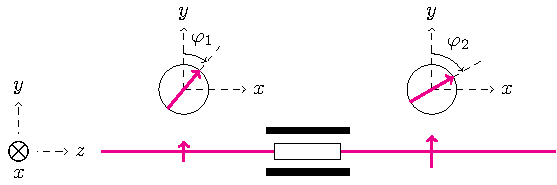
\includegraphics[width=0.8\textwidth]{images/rotpol}
	\end{center}
\end{frame}

%%%%%%%%%%%%%%%%%%%%%%%%%%%%%%%%%%%%%%%%%%%%%%%%%%%%%%%%%%%%%

\begin{frame}[t]
	\subsection{Вращатели Фарадея}
	%
	\frametitle{Вращатель и изолятор Фарадея}
	% \framesubtitle{Вращение плоскости поляризации}
	\textbf{Вращатель Фарадея} - устройство, способное вращать плоскость поляризации в магнитном поле. \textbf{Изолятор Фарадея} - устройство, поворачивающее плоскость поляризации на $\frac{\pi}{4}$. 
	% \vspace{1em}
	\begin{center}
		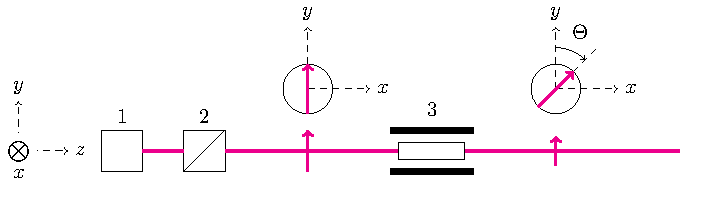
\includegraphics[width=0.8\textwidth]{images/rot}\\
		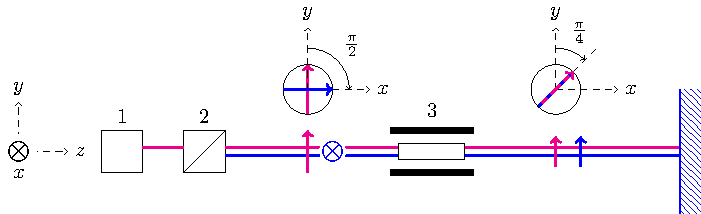
\includegraphics[width=0.8\textwidth]{images/zerc}
	\end{center}
	\begin{columns}
		\hspace{2.5cm}
		\begin{column}{0.3\textwidth}
			
			\textbf{1} -- источник
			
			\textbf{2} -- поляризатор
			
		\end{column}
		\hspace{1.6cm}
		\begin{column}{0.7\textwidth}
			
			\textbf{3} -- вращатель\\
			или изолятор Фарадея
		\end{column}
	\end{columns}
\end{frame}

%%%%%%%%%%%%%%%%%%%%%%%%%%%%%%%%%%%%%%%%%%%%%%%%%%%%%%%%%%%%%

\section{Экспериментальная часть}
\begin{frame}
	\subsection{Схема установки}
	\frametitle{Схема установки}
	\begin{figure}[tb]
		\centering
		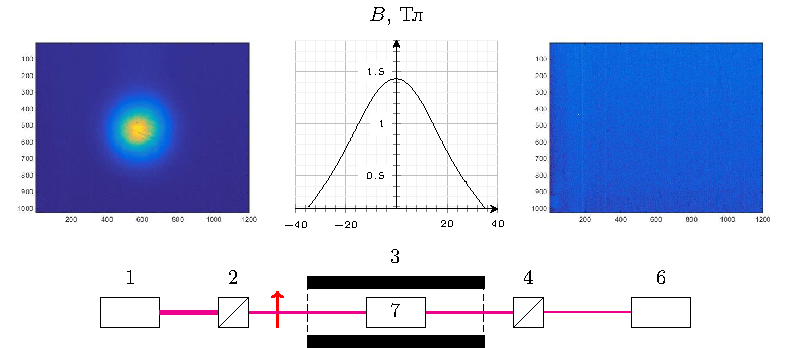
\includegraphics[width=1\textwidth]{images/chem}
	\end{figure}
	\begin{columns}
		\hspace{2.5cm}
		\begin{column}{0.3\textwidth}
			\textbf{1} -- диодный лазер\\ 
			$\quad\lambda_1=531$ нм,\\
			$\quad\lambda_2=658$ нм,\\
			$\quad\lambda_3=1064$ нм\\
			\textbf{2} -- поляризатор
		\end{column}
		\hspace{1.6cm}
		\begin{column}{0.7\textwidth}
			\textbf{3} -- магнит\\
			\textbf{4} -- призма Глана\\
			\textbf{5} -- фильтр\\
			\textbf{6} -- камера\\
			\textbf{7} -- образец
		\end{column}
	\end{columns}
\end{frame}

%%%%%%%%%%%%%%%%%%%%%%%%%%%%%%%%%%%%%%%%%%%%%%%%%%%%%%%%%%%

\begin{frame}
	\subsection{Аппроксимация распределения магнитного поля}
	\frametitle{Аппроксимация распределения магнитного поля}
	Аппроксимация распределение $B(z)$ с помощью кривой Гаусса:\vspace{-1em}
	\begin{columns}
		\begin{column}{0.6\textwidth}
			\begin{center}
				\hspace{4em}
				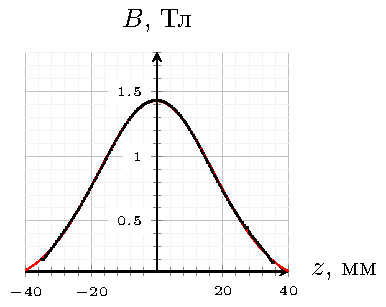
\includegraphics[width=\textwidth]{images/b_from_z}
			\end{center}
		\end{column}
		\begin{column}[]{0.4\textwidth}
			\begin{equation*} 
				B=B_0%\frac{1}{\sigma\sqrt{2\pi}} 
				\exp 
				\left[
					-\left(
					\frac{z-z_0}{c}
					\right)^2
					% - (x-\mu)^2
					% \cdot
					% B^2_0\pi 
					\right], 
			\end{equation*}
			где 
			
			$B_0=1.43$ Тл, \\
			$z_0=-0.25$ мм,\\
			$c=25$ мм.
		\end{column}
	\end{columns}
	%$\mu=-0.2581\pm0.03$, $\sigma=17.72\pm0.05$
	% ЗАМЕНИТЬ КОНСТАНТЫ ВВЕСТИ В0 НАПИСАТЬ РАЗМЕРНОСТИ
	% $	a1 = 1.428;%  (1.425, 1.43)
	% b1 = -0.2581;%  (-0.2927, -0.2235)
	% c1 = 25.06;%  (25, 25.11)
	% FF=@(x)  a1.*exp(-((x-b1)./c1).^2);$
\end{frame}

%%%%%%%%%%%%%%%%%%%%%%%%%%%%%%%%%%%%%%%%%%%%%%%%%%%%%%%%%%

\begin{frame}[t]
	\subsection{Анализ результатов}
	\frametitle{Результаты эксперимента}

	\vspace{-1em}
	\begin{figure}[tb]
		\centering
		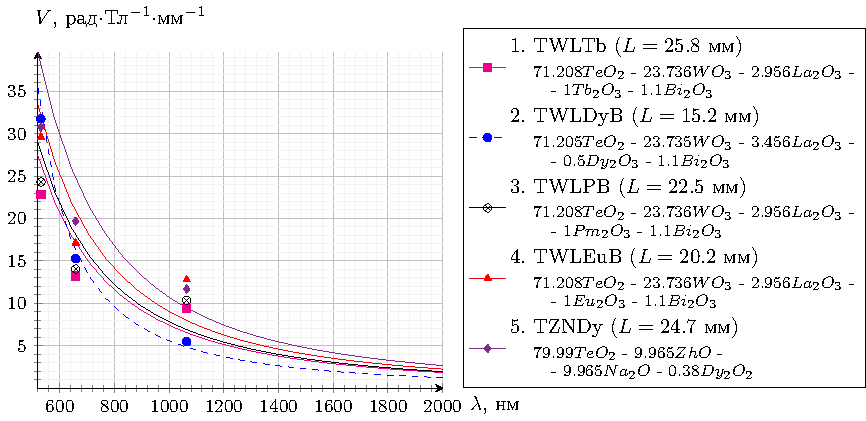
\includegraphics[width=1\textwidth]{images/graph_verde_from_lambda2}
	\end{figure}
	\vspace{-1em}
	\begin{equation*}
		V=
		% \frac{1}{\lambda}\left(
		% A+
		\frac{A}{\lambda^2-\lambda_0^2}
		% \right)
	\end{equation*}	
	\textbf{Оценка} образца TZNDy-236/4: Для поворота на $\Theta=\frac{\pi}{4}$ при $B=3.5$ Тл и длине волны $\lambda=1800$ нм нужен образец длиной 2 см.
	
	% Для оценки был выбран образец с наибольшей материальной константой, так как он на наибольший угол поворачивает плоскость поляризации.
	
	%Длина образца с составом TZNDy-236/4, при которой плоскость поляризации повернулась бы на $\frac{\pi}{4}$ -- 2см для волны 1,8мкм.
	
	%При такой длине образца неоднородность магнитного поля сказываться не будет, следовательно, как изолятор Фарадея его эффективно применять при таком магнитном поле.
\end{frame}

%%%%%%%%%%%%%%%%%%%%%%%%%%%%%%%%%%%%%%%%%%%%%%%%%%%%%%%%%%

\section{Выводы}
\begin{frame}
	\frametitle{Выводы}
	% В этой работе 
	\begin{enumerate} 
		\item 
			  Ознакомились с принципом работы вращателей и изоляторов Фарадея
		\item 
		      Исследовали магнитооптические свойства теллуритных стекол (определили постоянную Верде)
		\item 
		      Оценили длину образца, который можно использовать в качестве магнитооптического материала в изоляторах Фарадея, работающих в среднем ИК-диапазоне.
		      % ИК потому, что...ё
	\end{enumerate}
\end{frame}

%%%%%%%%%%%%%%%%%%%%%%%%%%%%%%%%%%%%%%%%%%%%%%%%%%%%%%%%%%

\begin{frame}[plain]
	\vspace{4cm}
	\begin{center}
		\Huge
		Спасибо за внимание!
	\end{center}
	\vspace{2.5cm}
	\begin{center}
		\color{black!30!white}
		Презентация подготовлена в издательской \\
		системе LaTeX с использованием пакетов \\
		PGF/TikZ и Beamer
	\end{center}
\end{frame}

%%%%%%%%%%%%%%%%%%%%%%%%%%%%%%%%%%%%%%%%%%%%%%%%%%%%%%%%%%

\begin{frame}
	\frametitle{Сложение взаимно перпендикулярных гармонических колебаний}
	Рассмотрим уравнение волны: 
	\begin{gather*} 
		\begin{cases} 
			E_x = E_1\cos\left(-kz+\omega t+\varphi_1\right) \\ 
			E_y = E_2\cos\left(-kz+\omega t+\varphi_2\right) \\ 
			E_z = 0 
		\end{cases}
	\end{gather*}
	Исключим из них время. Для этого 
	\begin{enumerate} 
		\item % 
		      $\frac{E_x}{E_1}=\cos(-{k}{z}+\omega t)\cos\varphi_1-\sin(-kz+\omega t)\sin\varphi_1$\\ %(*) 
		      $\frac{E_y}{E_2}=\cos(-kz+\omega t)\cos\varphi_2-\sin(-kz+\omega t)\sin\varphi_2$ %(**) 
		\item 
		      %Умножив выражение (*) на $\cos\varphi_2$ и (**) на $\cos\varphi_1$ после вычитания из первого равенства второго, получим: 
		      $\frac{E_x}{E_1}\cos\varphi_2-\frac{E_y}{E_2}\cos\varphi_1=\sin(-kz+\omega t)\sin(\varphi_2-\varphi_1)$
		\item 
		      %Теперь умножим выражение (*) на $\sin\varphi_2$ , а (**) на $\sin\varphi_1$ и также вычтем з первого равенства второе 
		      $\frac{E_x}{E_1}\sin\varphi_2-\frac{E_y}{E_2}\sin\varphi_1=\sin(-kz+\omega t)\sin(\varphi_2-\varphi_1)$
		\item 
		      %Возведя в квадрат и сложив почленно последние два уравнения, получим уравнение траектории 
		      $\frac{E_x^2}{E_1^2}-\frac{2E_xE_y}{E_1E_2}\cos(\varphi_2-\varphi_1)+\frac{E_y^2}{E_2^2}=\sin(\varphi_2-\varphi_1)$, 
		      $\varphi_2-\varphi_1=\delta$
		\item $\frac{E_x^2}{E_1^2}-\frac{2E_xE_y}{E_1E_2}\cos\delta+\frac{E_y^2}{E_2^2}=\sin^2\delta$
	\end{enumerate}
	% А это уравнение эллипса.
	% Следовательно, поляризация в общем случае эллиптическая. 
\end{frame}

%%%%%%%%%%%%%%%%%%%%%%%%%%%%%%%%%%%%%%%%%%%%%%%%%%%%%%%%%%

\begin{frame}

	\frametitle{Поворот поляризации}
	\begin{enumerate} 
		\item
		      Для простоты предположим, что начальная фаза волны равна нулю.
		      \begin{gather*}
			      \begin{cases} 
				      E_x = A\cos(\xi)\cos\left(-kz+\omega t\right) \\
				      E_y = A\sin(\xi)\cos\left(-kz+\omega t\right)
			      \end{cases}
		      \end{gather*}
		\item
		      Предположим, что поворот поляризации линейно зависит от $z$:
		      \begin{equation*}
			      \xi=-\alpha z
		      \end{equation*}
		      \begin{gather*}
			      \begin{cases} 
				      E_x = \frac{A}{2}\left[
					      \cos\left(
					      \xi+kz-\omega t
					      \right)+
					      \cos\left(
					      \xi-kz+\omega t
					      \right)
					      .\right] \\
				      E_y = \frac{A}{2}\left[
					      \sin\left(
					      \xi-kz+\omega t
					      \right)+
					      \sin\left(
					      \xi+kz-\omega t
					      \right)
					      \right]
			      \end{cases}
		      \end{gather*}
		\item
		      \begin{gather*}
			      \begin{cases} 
				      E_x = \frac{A}{2}\left[
					      \cos\left(
					      -z(k-\alpha)+\omega t
					      \right)+
					      \cos\left(
					      -z(k+\alpha)+\omega t
					      \right)
					      \right] \\
				      E_y = \frac{A}{2}\left[
					      \cos\left(
					      -z(k-\alpha)+\omega t+\frac{\pi}{2}
					      \right)+
					      \cos\left(
					      -z(k+\alpha)+\omega t-\frac{\pi}{2}
					      \right)
					      \right]
			      \end{cases}
		      \end{gather*}
	\end{enumerate}
\end{frame}


\begin{frame}
	\begin{enumerate} 
		\setcounter{enumi}{3}
		\item
		      Представим через суперпозицию, где $k^R=k-\alpha$, $k^L=k+\alpha$:
		      \begin{gather*}
			      \begin{cases}
				      \begin{cases} 
					      E_x^R = \frac{A}{2}
					      \cos\left(
					      \omega t - k^Rz
					      \right)
					      \\
					      E_y^R = \frac{A}{2}
					      \cos\left(
					      \omega t - k^Rz +\frac{\pi}{2}
					      \right)
				      \end{cases}\vspace{0.5em} \\
				      \begin{cases} 
					      E_x^L = \frac{A}{2}
					      \cos\left(
					      \omega t - k^Lz
					      \right)
					      \\
					      E_y^L = \frac{A}{2}
					      \cos\left(
					      \omega t - k^Lz -\frac{\pi}{2}
					      \right)
				      \end{cases}
			      \end{cases}
		      \end{gather*}
		      \begin{equation*}
			      \omega=2\pi\nu,\quad
			      \lambda=\frac{2\pi}{k},\quad\Rightarrow\quad
			      v=\lambda\nu=\frac{\omega}{k}
		      \end{equation*}
		\item
		      Тогда выразим скорости и показатели преломления этих волн:
		      \begin{gather*}
			      v_L=\frac{\omega}{k-\alpha},
			      \quad
			      v_R=\frac{\omega}{k+\alpha},
			      \quad
			      n_L=\frac{c}{v_L},
			      \quad
			      n_R=\frac{c}{v_L}
		      \end{gather*}
		      откуда 
		      \begin{equation*}
			      n_L-n_R=\frac{2c}{\omega}\alpha
		      \end{equation*}
		\item
		      \begin{equation*}
			      \alpha=\frac{\omega}{2c}(n_L-n_R)
		      \end{equation*}
	\end{enumerate}
\end{frame}

%%%%%%%%%%%%%%%%%%%%%%%%%%%%%%%%%%%%%%%%%%%%%%%%%%%%%%%%%%%%%
\end{document}

1. влияние состава стекол
влияет примесь .
Размер - апертура (какой размер, сколько можно) (до 10 и слава богу)
